% document class and packages
\documentclass[12pt,notitlepage]{report}
\usepackage{bibunits}
%\usepackage{hyperref}
\usepackage{uwmthesis}
\usepackage{graphicx}
\usepackage{subfigure}
\usepackage{color}
\usepackage{amsmath}
\usepackage{amssymb}
\usepackage{amsfonts}
\usepackage{acronym}

% journal definitions
\newcommand{\apj}{{\it Astrophysical J.}}
\newcommand{\apjl}{{\it Astrophysical J.}}
\newcommand{\aap}{{\it Astron. and Astrophys.}}
\newcommand{\cmp}{{\it Commun. Math. Phys.}}
\newcommand{\grg}{{\it Gen. Rel. Grav.}}
\newcommand{\cqg}{{\it Class. Quant. Grav.}}
\newcommand{\lr}{{\it Living Reviews in Relativity}}
\newcommand{\mnras}{{\it Mon. Not. Roy. Astr. Soc.}}
\newcommand{\pr}{{\it Phys. Rev.}}
\newcommand{\prl}{{\it Phys. Rev. Lett.}}
\newcommand{\prd}{{\it Phys. Rev. D}}
\newcommand{\prsl}{{\it Proc. R. Soc. Lond. A}}
\newcommand{\ptrsl}{{\it Phil. Trans. Roy. Soc. London}}
\newcommand{\rmp}{{\it Rev. Mod. Phys.}}

% acronymn definitions
\acrodef{LIGO}{Laser Interferometer Gravitational-wave Observatory}
\acrodef{BNS}{binary neutron star}
\acrodef{BBH}{binary black hole}
\acrodef{NSBH}{neutron-star black-hole binary}
\acrodef{FAR}{\emph{false alarm rate}}
\acrodef{SNR}{signal-to-noise ratio}
\acrodef{MM}{minimal match}
\acrodef{IFO}{interferometer}
\acrodef{CBC}{compact binary coalesence}
\acrodef{GW}{gravitational wave}
\acrodef{PDF}{probability distribution function}
\acrodef{PSD}{power spectral density}
\acrodef{S5}{LIGO's fifth science run}
\acrodef{S6}{LIGO's sixth science run}
\acrodef{pN}{post-Newtonian}

% common macros
\def\Msun{\ensuremath{\mathrm{M_\odot}}}
\def\Mpc{\ensuremath{\,\mathrm{Mpc}}}
\def\yr{\ensuremath{\,\mathrm{yr}}}
\def\mchirp{\ensuremath{\mathcal{M}}}
\def\mtotal{\ensuremath{\mathrm{M_{total}}}}
\def\d{\ensuremath{\,\mathrm{d}}}
\def\pls{\ensuremath{+}}
\def\crs{\ensuremath{\times}}
\def\effD{\ensuremath{\mathcal{D}}}
\def\th{\ensuremath{^{\mathrm{th}}}}

\begin{document}
\title{% taken from dissertator fellowship application
Searching for Gravitational Waves from Compact Binary Coalescence in S6
}
\author{\bf Collin D. Capano}
\majorprof{Duncan A. Brown}
\submitdate{August 2011}
\degree{Doctor of Philosophy}
\program{Physics}

\Chapter{Obtaining Gravitational Wave Triggers from Interferometer Data}
\label{ch:pipeline_principles}
Using General Relativity we were able to write down an expression for the strain induced in an interferometer from a passing gravitational wave. In this chapter we detail how to detect gravitational-wave signals from \acp{CBC} in the interferometer data in the presence of noise. We begin by deriving the \emph{matched filter} for a single template, which is the optimal filter if the detector noise is stationary and Gaussian. Next, we show how matched filtering can be done for a bank of templates in order to recover the parameters of a signal. This is followed by a discussion of the $\chi^2$ test, which can be used to suppress triggers from non-Gaussian transients that are present in real detector data. Finally, we detail how a coincidence test can be done across multiple detectors to further decrease the number of false noise triggers produced by a search.

\section{Detecting a Gravitational Wave Using a Matched Filter}
\label{sec:matched_filter}

Equation \ref{eqn:non_spin_template} gave the strain, $h(t)$, induced in an \ac{IFO} when a gravitational-wave from an inspiraling compact binary with non-spinning component masses passes through. The strain was a function of chirp mass, $\mchirp$, and symmetric-mass ratio, $\eta$. If we wish to search for a gravitational wave that came from a binary with given $\mchirp$ and $\eta$, we can generate a waveform, or template, that characterizes it. We now address the question: if a gravitational wave that matches our template exists in the \ac{IFO} data, how do we find it?

Let the output of the detector be the time series $s(t)$, which is a measure of the displacement of the \ac{IFO}'s mirrors as a function of time. If a gravitational wave with waveform $h(t)$ exists in the data, then:

\begin{equation}
\label{eqn:ifo_data}
s(t) = h(t) + n(t)
\end{equation}
where $n(t)$ is the strain induced by all other, non gravitational-wave,  sources, or ``noise," as a function of time. If no signal exists in the data, then $s(t) = n(t)$. We do not know \emph{a priori} if $h$ exists in the data; further, even if $h$ does exist, we do not know \emph{when} it occurs --- that is, we do not know its coalescence time, $\tau_c$.\footnote{Note that the exact time when $h$ occurs is somewhat arbitrary. We could choose any point in the evolution of the waveform and label that as the point that $h$ occurs. For \ac{CBC} templates, we chose to use the time of coleascence since it is easily identifiable: it is the point that the \ac{pN} approximation goes to infinite frequency.} Our goal, then, is to find a filter that takes $s(t)$ and $h(t-\tau)$ as input and returns a number, $\rho(\tau)$, that is proportional to the probability that $h$ is in $s$ with coalescence time $\tau$, $P(h(t-\tau)|s(t))$. We additionally require that, if $h$ is in $s$, this filter is at a maximium at the point that $h$ occurs. If we have such a filter --- known as the \emph{optimal filter} --- then we can determine that a signal exists in the data if $\rho(\tau)$ exceeds some pre-determined threshold $\rho^{*}$. Further, we can determine the coalescence time of $h$ by simply incrementing $\tau$ and evaluating $\rho$ at each increment, selecting points when $\rho$ is at a maximum. (This is known as the method of maximum likelihood \cite{ref:Brown}.)

We begin by assuming that $\tau = \tau_c = 0$ and looking for the filter that maximizes $P(h|s)$ (for now, we will drop the ``$(t)$" for clarity). The problem of finding an optimal filter to extract signals from (Gaussian) noise is well studied, and has been applied to radar analysis for decades. Here, we follow the method outlined in \cite{ref:Finn,ref:Finn_Chernoff,ref:Brown} --- all of which use methods detailed in Wanstein and Zubakov \cite{ref:Wanstein_Zubakov} --- to derive the filter.

Using Bayes' theorem \cite{ref:Sivia} we can write $P(h|s)$ as:
\begin{equation}
\label{eqn:P_of_h1}
P(h|s) = \frac{P(s|h) P(h)}{P(s)}
\end{equation}
where:
\begin{eqnarray}
P(s|h) & \equiv & \mbox{the probability of getting $s$ if $h$ exists in it} \nonumber \\
P(h)   & \equiv & \mbox{the probability of the signal, $h$, occurring} \nonumber \\
P(s)   & \equiv & \mbox{the probability of getting $s$} \nonumber
\end{eqnarray}
Since the signal either does or does not exist in the data, the probability of getting a particular instance of $s$ is:
\begin{equation}
P(s) = P(s|0)P(0) + P(s|h)P(h)
\end{equation}
where:
\begin{eqnarray}
P(s|0) & \equiv & \mbox{the probability of getting $s$ if no signal exists} \nonumber \\
P(0) & \equiv & \mbox{the probability of getting no signal} \nonumber
\end{eqnarray}
Plugging this into \ref{eqn:P_of_h1} we have:
\begin{eqnarray}
\label{eqn:P_of_h}
P(s|h) & = & \frac{ P(s|h) P(h) }{ P(s|0)P(0) + P(s|h)P(h) } \nonumber \\
 & = & \frac{ P(s|h) } { P(s|0) \left(\, P(0)/P(h) + P(s|h)/P(s|0) \,\right) } \nonumber \\
 & = & \frac{ \Lambda }{ P(0)/P(h) + \Lambda }
\end{eqnarray}
where
\begin{equation}
\label{eqn:likelihood_ratio}
\Lambda \equiv \frac{ P(s|h) }{ P(s|0) }
\end{equation}
is the \emph{likelihood ratio}. $P(0)$ and $P(h)$ are known as \emph{priors}: they represent our \emph{a priori} belief that a signal does or does not exist, irrespective of the detector's ability to detect it. We do not need to concern oursevles with assigning values to them, however. Instead we note that $P(s|h)$ is a monotonically increasing function of $\Lambda$. Since we are only interested in a filter that maximizes $P(s|h)$, and not the exact value of $P(s|h)$, we can therefore limit our focus to evaluating $\Lambda$, and threshold on the point that it reaches a maximum. We further note that the natural logarithm of $\Lambda$ also increases monotonically with $P(s|h)$. Since we will be interested in evaluating the likelihood in the region that $\Lambda$ is a maximum, it is common practice to instead evaluate the \emph{log-likelihood}, $\ln \Lambda$, instead, as it is less ``peaky" around the region of interest \cite{ref:Sivia}.

Before calculating the log-likelihood, we note that we do not know \emph{a priori} the phase of the binary, $\theta$. Therefore, we treat $\theta$ as a \emph{nuisance} parameter, which we marginalize over \cite{ref:Sivia}. Thus, we write the likelihood ratio as:
\begin{eqnarray}
\Lambda & = & \int_0^{2 \pi} p(\theta) \lambda(\theta) \d\theta \nonumber \\
 & = & \frac{1}{2\pi P(s|0)} \int_0^{2 \pi} p(s|h(\theta)) \d\theta
\end{eqnarray}
Here, $\lambda(\theta)$ is the likelihood ratio at a given $\theta$, $p(\theta)$ is the prior probability of getting $\theta$, and we have written $P(s|h)$ as the \ac{PDF} $p(s|h(\theta))$; $P(s|0)$ remains outside of the integral as it has no $\theta$ dependence. Assuming any phase is eqaully likely, we set $p(\theta) = 1/2\pi$ and also pulled it out of the integral.

To calculate the likelihood ratio, we need $p(s|h(\theta))$ and $P(s|0)$. We focus first on $P(s|0)$. If $s(t)$ has no signal in it then it is simply $n(t)$. $P(s|0)$ is therefore the probability of getting a particular realization of the noise. Let us assume that the noise is a stationary Gaussian process with zero mean. For our purposes it will be useful to characterize the noise by its \ac{PSD}, $S_n(|f|)$ rather than its variance. The \ac{PSD} is defined as the Fourier Transform of the autocorrelation of the noise \cite{ref:Wainstein_Zubakov}:
\begin{equation}
S_n(|f|) \equiv \int_{-\infty}^{\infty} R(\tau)e^{-i 2\pi ft} \d t = \overline{\widetilde{n}^{*}(f)\widetilde{n}(f)}
\end{equation}
where,
\begin{equation}
R(\tau) = \overline{n(t)n(t-\tau)}
\end{equation}
is the autocorrelation function. Note that $R(0) = \overline{n(t)^2}$, which is the variance since $\overline{n(t)} = 0$. We restrict our analysis to positive frequencies; thus we will use the one-sided \ac{PSD} $S_n(|f|) = S_n(f)/2$. It is shown in \cite{ref:Finn} that with these assumptions, the probability of getting a given realization of the noise, $n = s$, is:
\begin{equation}
\label{eqn:p_no_sig}
P(s|0) = \alpha \exp[ - \frac{1}{2} (s|s) ]
\end{equation}
where $\alpha$ is a normalization constant and the inner-product $(\cdot|\cdot)$ is defined as:
\begin{eqnarray}
\label{eqn:inner_product1}
(a|b) & \equiv & \int_{-\infty}^{\infty} \frac{ \widetilde{a}^{*}(f)\widetilde{b}(f) + \widetilde{a}(f)\widetilde{b}^{*}(f) }{S_n(|f|)} \d f \\
\label{eqn:inner_product2}
 & = & 2 \int_{-\infty}^{\infty} \frac{ \widetilde{a}^{*}(f)\widetilde{b}(f) }{S_n(|f|)} \d f
\end{eqnarray}
In going from \ref{eqn:inner_product1} to \ref{eqn:inner_product2} we have used the fact that for real functions of time (which both $h$ and $s$ are), $\widetilde{g}^{*}(f) = \widetilde{g}(-f)$.

Using this result we can also find $p(s|h(\theta))$. If $h$ is in the data, then $n(t) = s(t) - h(t, \theta)$. Thus,
\begin{eqnarray}
\label{eqn:p_sig}
p(s|h) & = & \alpha \exp\{ -\frac{1}{2} (s - h | s - h ) \} \nonumber \\
 & = & \alpha \exp\{ -\frac{1}{2} [ (s|s) - 2(h|s) + (h|h) ] \} \nonumber \\
 & = & P(s|0) \exp\{ (h|s) - (h|h)/2 \}
\end{eqnarray}
Plugging \ref{eqn:p_no_sig} and \ref{eqn:p_sig} into \ref{eqn:likelihood_ratio}, the likelihood ratio becomes:
\begin{eqnarray}
\label{eqn:lambda1}
\Lambda & = & \frac{1}{2\pi} \int_0^{2\pi} \exp\{ (h|s)- \frac{(h|h)}{2} \} \d\theta \\
\label{eqn:lambda2}
 & = & \frac{1}{2\pi} e^{-(h|h)/2} \int_0^{2\pi} \exp\{ (~C(t)\cos(2\phi(t) - \theta)~|~s~) \} \d\theta
\end{eqnarray}
In going from \ref{eqn:lambda1} to \ref{eqn:lambda2} we have plugged in the general form of $h(t, \theta)$, which is given in equation \ref{eqn:general_h}. We have also pulled the $(h|h)$ term out of the integral as it is simply a number --- it is the inner product of $h$ with itself --- and has no phase dependence. In order to evaluate the integral, we re-write the inner product of $s$ with $h$ as follows:
\begin{eqnarray}
\label{eqn:sh_in_z}
(h|s) & = &  (~C(t) \cos(2\phi(t) - \theta)~|~s(t)~) \nonumber \\
 & = & (~C(t)\cos(2\phi(t))~|~s(t)~) \cos(\theta) + (~C(t)\sin(2\phi(t))~|~s(t)~) \sin(\theta) \nonumber \\
 & = & x \cos(\theta) + y\sin(\theta) \nonumber \\
 & = & |z|\cos(\Phi)\cos(\theta) + |z|\sin(\Phi)\sin(\theta) \nonumber \\
 & = & |z|\cos(\Phi - \theta)
\end{eqnarray}
where:
\begin{align}
\label{eqn:matchf_x}
x &= (~C(t)\cos(2\phi(t))~|~s(t)~) \equiv (h_{\pls}|s) \\
\label{eqn:matchf_y}
y &= (~C(t)\sin(2\phi(t))~|~s(t)~) \equiv (h_{\crs}|s) \\
|z| &= \sqrt{ x^2 + y^2 } \\
\Phi &=  \tan^{-1}\left( \frac{y}{x} \right) 
\end{align}
Since the \ac{GW} phase, $2\phi(t)$, is $90^{\circ}$ out of phase in equations \ref{eqn:matchf_x} and \ref{eqn:matchf_y}, we have identified $x$ and $y$ as the inner products of the plus and cross polarizations, respectively, with the data. Due to their orthogonality, note that:
\begin{align}
(h_\pls|h_\pls) &= (h_\crs|h_\crs) &= (h|h) \\
(h_\pls|h_\crs) &= (h_\crs|h_\pls) &= 0
\end{align}
Also note that we can let $z$ be complex:
\begin{equation}
z = x + iy
\end{equation}
This will prove useful below.

%Note that in this case we can write:
%\begin{align*}
%z &= (h_c|s) + i(h_s|s) \\
%  &= (h_c|s) + (-ih_s|s) \\
%  &= (h_c - ih_s|s) \\
%  &= (H|s)
%\end{align*}
%where $H$ is the phasor:
%\begin{equation}
%H(t) = C(t)e^{-i2\phi(t)}
%\end{equation}
%
%Using this formalism we can write:
%\begin{align}
%\label{eqn:matchf_xcmplx}
%x &= \Re(h|s) \\
%\label{eqn:matchf_ycmplx}
%y &= \Re (ih|s) \\
%\label{eqn:matchf_cmplx}
%z &=  (h|s) + i(h|s) \\
%\Rightarrow |z| &= \sqrt{2} (h|s)
%\end{align}
%Here $\Re$ denotes the real part of the functions. Using this complex notation will prove useful below.

Plugging equation \ref{eqn:sh_in_z} into the likelihood ratio, we have:
\begin{eqnarray}
\Lambda & = & \frac{1}{2\pi} e^{-(h|h)/2} \int_0^{2\pi} \exp\{ |z|\cos(\Phi - \theta) \} \d \theta \nonumber \\
 & = & e^{-(h|h)/2} I_0(|z|) \nonumber \\
\label{eqn:modBessel}
 & = & e^{-(h|h)/2} \sum_{k=0}^{\infty} \frac{(|z|^{2}/4)^{k}}{(k!)^2} \\
 \label{eqn:posDef}
 & \leq & e^{-(h|h)/2} \left( \sum_{k=0}^{\infty} \frac{ (|z|^{2}/4)^k }{k!} \right) \left(\sum_{m=0}^{\infty} \frac{1}{m!}\right) \\
 & \leq & e^{-(h|h)/2} e^{|z|^{2}/4 - 1}
\end{eqnarray}
where $I_0(|z|)$ is the modified Bessel function of the first kind, which is equal to the sum in equation \ref{eqn:modBessel} \cite{ref:Wolfram}. To go from equation \ref{eqn:modBessel} to \ref{eqn:posDef} we have used the fact that $(|z|^{2}/4)^{k}/k!$ and $1/k!$ are positive definite for all $k$. Thus, the likelihood ratio is maximized when it is equal to $\exp\{ |z|^2/4 + 1 - (h|h)/2 \}$, and so we can threshold when the log-likelihood is:
\begin{equation}
\ln \Lambda = \frac{1}{4}|z|^2 + 1 - \frac{1}{2}(h|h)
\end{equation}
The factor of $1/4$ and the $+1$ term on the right-hand side of the equation only scale and offset $\ln\Lambda$ by constants. We can therefore threshold on:
\begin{equation}
4 \ln \Lambda - 4 = |z|^2 - 2(h|h)
\end{equation}
instead, without any loss in ability to detect $h$. The $(h|h)$ term, however, causes the log-likelihood to be template dependent. Since we will be filtering multiple templates, we prefer to use a quantity that is independent of the template used. Therefore, we normalize both sides by $(h|h)$. Dropping the remaining $-2$ offset, we are left with:
\begin{equation}
\frac{|z|^2}{(h|h)} \equiv \rho^{2}
\end{equation}
The quantity $\rho^2$ is our detection statistic.

In the absence of a signal, $(h|h)$ is the variance of the filter. To see this, first note that the mean of $(h|n)$ is zero:
\begin{eqnarray}
\overline{(h|n)} & = & 2 \overline{\int_{-\infty}^{\infty} \frac{\widetilde{h}^{*}(f)\widetilde{n}(f)}{S_n(|f|)} \d f} \nonumber \\
 & = & 2 \int_{-\infty}^{\infty} \frac{\widetilde{h}^{*}(f)\overline{\widetilde{n}(f)}}{S_n(|f|)} \d f \nonumber \\
 & = & 0
\end{eqnarray}
since $\overline{n(t)} = \overline{\widetilde{n}(f)} = 0$. The mean of the square of $(h|n)$ is:
\begin{eqnarray}
\overline{(h|n)^2} & = & \overline{\left| 2 \int_{-\infty}^{\infty} \frac{\widetilde{h}^{*}(f)\widetilde{n}(f)}{S_n(|f|)} \d f \right|^2 } \nonumber \\
 & = & 4 \int_{-\infty}^{\infty} \int_{-\infty}^{\infty} \frac{\widetilde{h}(f')\widetilde{h}^{*}(f)\overline{\widetilde{n}^{*}(f')\widetilde{n}(f)}}{S_n(|f'|)S_n(|f|)} \d f' \d f \nonumber \\
 & = & 4 \int_{-\infty}^{\infty} \int_{-\infty}^{\infty} \frac{\widetilde{h}(f')\widetilde{h}^{*}(f) S_n(|f'|)\delta(f'-f)}{2 S_n(|f'|)S_n(|f|)} \d f' \d f \nonumber \\
 & = & 2 \int_{-\infty}^{\infty} \frac{\widetilde{h}(f)\widetilde{h}(f)}{S_n(|f|)} \d f \nonumber \\
 & = & (h|h)
\end{eqnarray}
Thus the variance is:
\begin{equation}
\sigma^2 = \overline{(h|n)^2} - \overline{(h|n)}^2 = (h|h)
\end{equation}
and we can write:
\begin{equation}
\label{eqn:SNR}
\rho^2 = \frac{|z|^2}{\sigma^2}
\end{equation}
We therefore identify $\rho$ as the \emph{\ac{SNR}} of the template.

In order to evaluate $\rho$ for arbitrary values of $\tau \neq \tau_c \neq 0$, we note that the Fourier Transform of $h(t-\tau)$ is: 
\begin{eqnarray}
\widetilde{h}(f) & = & \int_{-\infty}^{\infty} h(t-\tau) e^{-i 2\pi f t} \d t \nonumber \\
& = & e^{i 2\pi f \tau} \int_{-\infty}^{\infty} h(t') e^{-i 2\pi ft'} \d t' \nonumber \\
& = & e^{i 2\pi f \tau} \widetilde{h}(f')
\end{eqnarray}
$\widetilde{h}(f')$ is the Fourier Transform of $h(t)$ independent of the coalescence time. We can thereby account for the unknown coalescence time by filtering:
\begin{equation*}
e^{-i 2\pi f\tau} \widetilde{h}(f)
\end{equation*}
This introduces a time-dependence to $\rho$:
\begin{align}
\rho(\tau)^2 &= \frac{|z(\tau)|^2}{\sigma^2} \nonumber \\
 &= \frac{1}{\sigma^2}\left( (h_{\pls}(\tau)|s)^2 + (h_{\crs}(\tau)|s)^2 \right) \nonumber \\
\label{eqn:snr_full_form}
 &= \frac{1}{\sigma^2}\left\{ \left( \int_{-\infty}^{\infty} \frac{\widetilde{h}_{\pls}^{*}(f)\widetilde{s}(f)}{S_n(|f|)} e^{i 2\pi f\tau} \d f \right)^2 + \left( \int_{-\infty}^{\infty} \frac{\widetilde{h}_{\crs}^{*}(f)\widetilde{s}(f)}{S_n(|f|)} e^{i 2\pi f\tau} \d f \right)^2 \right\}
\end{align}
To carry out the maximum likelihood operation, we create a \ac{SNR} time series by incrementing $\tau$ and filtering using equation \ref{eqn:snr_full_form} at each step. We then select points where $\rho(t)$ is a maximum; if the \ac{SNR} of a maximum point exceeds our pre-determined threshold we save it. Each of the saved events is a \emph{trigger}.

Now that we have established the \ac{SNR} as our detection statistic, let us examine a few important properties of it. In the absence of a signal ($s = n$) $\rho$ is $\chi^2$ distributed with two degrees of freedom; the squared mean is:
\begin{align}
\overline{\rho^2} &= \frac{1}{\sigma^2}\left( \overline{(h_{\pls}|n)^2} + \overline{(h_{\crs}|n)^2} \right) \nonumber \\
 &= \frac{ \left( (h_{\pls}|h_{\pls}) + (h_{\crs}|h_{\crs}) \right)}{(h|h)} \nonumber \\
 &= 2
\end{align}
since $(h_{\pls}|h_{\pls}) = (h_{\crs}|h_{\crs}) = (h|h)$. If we had only filtered one of the phases, $\overline{\rho^2}$ in noise would be 1. While filtering both $h_{\pls}$ and $h_{\crs}$ allowed us to account for the unknown phase, we have paid for our ignorance by doubling the noise floor. Our threshold for keeping triggers must therefore be larger than $\rho^{2} = 2$, as it is impossible to distinguish noise from triggers at or below this value.

As seen in equation \ref{eqn:h_general}, $h$ is inversely proportional to the effective distance to the binary, $\effD$. We can exploit this to relate $\effD$ to the \ac{SNR}. Assume the data only contains a signal (and no noise), i.e., $s = h'_{\pls}$, from a binary that has an effective distance of $\effD'\Mpc$. For simplicity we also assume the signal is plus-polarized with coalesence time $\tau_c = 0$. The templates we filter with are generated at a canonical distance of $1\Mpc$; therefore $h'_{\pls} = \effD'^{-1}h_{\pls}$. The \ac{SNR} would be:
\begin{align*}
\rho^2 &= \frac{1}{\sigma^2}\left( (h_{\pls}|h'_{\pls})^2 + (h_{\crs}|h'_{\pls})^2 \right) \\
 &= \frac{1}{\sigma^2} \left( \effD'^{-2}(h_{\pls}|h_{\pls})^2 + \effD'^{-2}(h_{\crs}|h_{\pls})^2 \right) \\
 &= \effD'^{-2} \sigma^2
\end{align*}
Thus:
\begin{equation}
\label{eqn:DtoRho}
\effD = \frac{\sigma}{\rho}
\end{equation}
Since $\sigma$ is inversely proportional to $\sqrt{S_n(|f|)}$, we see that it is a measure of the sensitivity of the detector. The noisier the detector is, the smaller $\sigma$ is, and so for a given \ac{SNR}, the range that we can detect will be smaller.

If the detector output is Gaussian, as we have assumed above, then we could relate \ac{SNR} directly to false alarm rate, and we could simply set the \ac{SNR} threshold based on some desired false alarm rate. Any trigger with a \ac{SNR} above that threshold would be considered a gravitational wave. However, as we will see in section \ref{sec:chisq}, the real detectors have high rates of non-Gaussian transients (``glitches") for which we have no model. We therefore have to measure the false alarm rate directly. How this is done is discussed in chapter \ref{ch:far}.

Finally, we will find it useful to define the complex form of the \ac{SNR} using the complex form of $z$ given in equation \ref{eqn:complex_z}:
\begin{align}
\varrho &= \frac{z}{\sigma} \nonumber \\
 &= \frac{(h_\pls|s) + i(h_\crs|s)}{(h|h)} \\
\rho &= |\varrho|
\end{align}
We will use this complex form in the $\chi^2$ test, discussed below.

\section{Filtering with Multiple Templates}
\label{sec:multiple_templates}
In the above section we assumed that the signal we were looking for had the same parameters as the template we used to search for it. We now address how to search for signals across a range of chirp masses and symmetric-mass ratios --- collectively known as \emph{instrinsic} parameters --- so that we can search for signals from many types of systems. Alternatively, if one signal exists in the data, we can think of this question as addressing how to estimate its parameters.

In order to find the intrinsic parameters we use a discreet \emph{bank} of templates. The templates are laid out in the bank by computing how quickly the inner product --- or \emph{overlap}, $\mathcal{O}$ --- between a template with intrinsic parameters $\theta_\mu$ and one with parameters $\theta_\mu + \Delta\theta_\mu$ falls off with increasing $\Delta\theta_\mu$. This is done by expanding the overlap around $\Delta\theta_\mu = 0$ \cite{ref:Owen:1995,ref:OwenSathya:1998,ref:Babak.et.al:2006}:

\begin{eqnarray}
\label{eqn:OverlapSeries}
\mathcal{O} & \equiv & \left( h(\theta_\mu) | h(\theta_\mu + \Delta\theta_\mu) \right)  \\
        & = & 1 + \frac{1}{2} \left.\frac{\partial^2\mathcal{O}}{\partial \Delta\theta^\mu \partial \Delta\theta^\nu} \right|_{\Delta\theta^\kappa = 0} \Delta\theta^\mu \Delta\theta^\nu + \ldots \nonumber \\
        & \approx & 1 - g_{\mu \nu}\Delta\theta^\mu\Delta\theta^\nu
\end{eqnarray}

where 

\begin{equation}
\label{eqn:templateMetric}
g_{\mu \nu} = -\frac{1}{2} \left.\frac{\partial^2\mathcal{O}}{\partial \Delta\theta^\mu \partial \Delta\theta^\nu} \right|_{\Delta\theta^\kappa = 0}
\end{equation}

$g_{\mu\nu}$ is the metric on the parameter space around the point $\theta_\mu$; it gives the ``distance" between two templates with slightly different parameters in terms of how much \ac{SNR} will be lost from their mis-match. Using the metric we can determine how many templates to place in a region of parameter space for an acceptable loss in \ac{SNR} due to the discretization. We quantify this by defining the \emph{\ac{MM}} \cite{ref:Owen:1996}, given by \cite{ref:Cokelaer:2007}:
\begin{equation}
\label{eqn:min_match}
\underset{\theta^\mu}{\min}~\underset{i}{\max}~(h(\theta^{\mu}_{i})|h'(\theta^{\mu})) \geq MM
\end{equation}
where $i \in \{ 1, 2, \ldots N_{\mathrm{templates}} \}$, $\mu \in \{ 1, 2, \ldots N_{\mathrm{parameters}} \}$, and $h'(\theta^{\mu})$ is the waveform of the signal in the data. In other words, the bank should be constructed such that there exists at least one template for which the match between it and any signal with parameters $\theta^\mu$ is $\geq MM$. We can use equation \ref{eqn:DtoRho} to determine an acceptable $MM$. For example, if $MM = 0.97$, then the maximum loss in \ac{SNR} for a signal that falls between two templates is $3\%$. The loss in effective range will be also be $3\%$, which translates to a loss in volume of $(\delta \effD)^3 = 9\%$. Choosing a larger $MM$ may appear to increase the range. However, a larger $MM$ increases the number of templates needed, and this must be weighed against computational cost and false alarm rate. The more templates we filter with, the higher the probability of getting accidental triggers from noise. This also decreses the sensitive volume as the \ac{SNR} at which we could claim a confident detection would have to increase. A $MM = 0.97$ is the currently used limit in \ac{CBC} searches.

If an analytic solution exists for the waveform in terms of the parameters $\theta_\mu$, then the metric can be evaluated directly to figure out the number of templates needed and where to place them. Laying the templates so that the overlap remains the same across the bank is best done in a coordinate system which is largely flat across the parameter space. This limits the number of parameters that can be accounted for, and it makes it more difficult to lay templates using higher-order \ac{pN} expansions, as the terms become larger and more complex. Currently, the metric has been computed for $2\,$\ac{pN} non-spinning templates, which are laid out on a hexagonal grid in $\tau_0$ and $\tau_3$ space. These are given by \cite{ref:Babak.et.al:2006}:
\begin{equation}
\label{eqn:tau0tau3}
\tau_0 = \frac{5}{256\pi f_0 \eta}(\pi \mtotal f_0)^{-5/3}, \quad \tau_3 = \frac{1}{8 f_0 \eta}(\pi \mtotal f_0)^{-2/3}
\end{equation}
where $f_0$ is the lower cutoff frequency of the template. We use $\tau_0$ and $\tau_3$ because the metric at $2\,$\ac{pN} is roughly flat in these coordinates \cite{ref:Babak.et.al:2006}. Hexagonal gridding --- as opposed to square gridding --- allows the space to be covered efficiently using a minimal number of templates \cite{ref:Cokelaer:2007}. Once the templates are laid out we can convert to $\mtotal$ and $\eta$ by inverting equations \ref{eqn:tau0tau3} to obtain \cite{ref:Babak.et.al:2006}:
\begin{equation}
\mtotal = \frac{5}{32\pi^2 f_0}\frac{\tau_3}{\tau_0}, \quad \eta = \frac{1}{8\pi f_0 \tau_3}\left(\frac{32\pi \tau_0}{5\tau_3}\right)^{2/3}
\end{equation}
See chapter \ref{ch:ihope_pipeline} for a plot of a typical template bank used in \ac{S5} and \ac{S6}.

Limiting the search to non-spinning templates means we cannot detect \acp{GW} from binaries with spinning component masses as well. In parameter space a spinning binary will live in a region above the non-spinning plane. This means the \ac{SNR} we obtain will be from the projection of the signal onto the non-spinning plane. The resulting loss in \ac{SNR} leads to a decrease in sensitivity to spinning signals. It has been shown that spin should not be much of a concern for \ac{BNS} systems \cite{ref:?}, as the component masses are too small to spin fast enough relative to the total angular momentum to have an affect on the \ac{GW}. However, spin does have a stronger effect on \ac{NSBH} and \ac{BBH} systems \cite{ref:?}. In \ac{S5} and \ac{S6} we estimated the effect of the spin of these systems on our ability to detect; see chapter \ref{ch:results} for details. Investigations into how to expand the template bank into non-spinning regions without substantially increasing the false alarm rate are on-going.

\section{The $\chi^2$ Test}
\label{sec:chisq}

Up to this point we have assumed that the detector output in the absence of a signal is stationary Gaussian noise. Unfortunately, the real detectors have a number of non-Gaussian glitches due to various instrumental and environmental factors. For example, train tracks are close enough to the \ac{LIGO} Livingston Observatory that when a freight train passes through it causes transients in the noise through seismic up-conversion \cite{ref:?}. Although these glitches do not have the same morphology as a gravitational wave from a \ac{CBC}, they do cause the matched-filter to ``ring off" high-\ac{SNR} triggers. Figure \ref{fig:snr_hist} shows a histogram of trigger counts as a function of \ac{SNR} ($\rho$) taken from H1 during two weeks of \ac{S6}. For reference, a $\chi^2$ distribution with two degrees of freedom --- expected if the detector noise is Gaussian --- is shown. Clearly, a large non-Gaussian tail is present in the data.

To better discriminate betwen potential signals and noise, we employ a $\chi^2$ test \cite{ref:Allen:2006}. The basic idea of this test is relatively straight-forward. Although a glitch can cause a trigger with the same (or larger) \ac{SNR} as a signal, the manner in which the \ac{SNR} is accumulated over time and frequency will most likely differ. For example, a delta function-like glitch will have a burst of power in a small window in the time domain, and the power will be smeared out across all frequencies. A \ac{CBC} \ac{GW}, on the other hand, will accumulate its power across the duration of the template, and it will do so in a ``chirping" manner. Therefore, if we break the template into frequency bins of equal power, filter each of these sub-templates, and compare the \ac{SNR} in each bin to the expected value, we can better discriminate glitch from signal.

Define a set of $p$ matched filters such that the $i\th$ filter is carried out between the frequencies $f_i$ and $f_{i+1}$:
\begin{equation}
(h_i|s) = \int_{f_i}^{f_{i+1}} \frac{ \widetilde{h}^{*}(f) s(f) }{S_n(|f|)} \d f, \quad i \in \{0~ \ldots~ p-1\},~ f \in \left[ f_0, f_{\mathrm{isco}} \right]
\end{equation}
(Note that on the left-hand side of the equation we put the $i$ index on $h$. This is because we could equally as well have broken the template up into each frequency bin, then filter each sub-template across the entire frequency range.) Each frequency bin is chosen so that the template has equal amounts of power in each bin. The amount of \ac{SNR} accumulated in one bin is thus:
\begin{align}
\rho_i &= \sqrt{\frac{(h_{\pls \,i}|s)^2 + (h_{\crs \,i}|s)^2}{(h|h)}} \nonumber \\
 &= \frac{1}{p} \rho
\end{align}
where $\rho$ is the total \ac{SNR}. We can therefore check how well the measured \ac{SNR} matches the expected \ac{SNR} in a single bin by:
\begin{equation*}
\Delta \rho_i = \rho_i - \frac{\rho}{p}
\end{equation*}
To check the match across the entire template, we define the $\chi^2$ test as \cite{ref:Allen}:
\begin{equation}
\label{eqn:basic_chisq}
\chi^2 = p \sum_{i=1}^{p} \left|\varrho_i - \frac{\varrho}{p}\right|^2
\end{equation}
Note that we have used the complex form of the \ac{SNR}, defined in equation \ref{eqn:complex_rho}, and we took the modulus after the subtraction. This is done so we can directly compare each polarization of the phase between the measured and the expected \acp{SNR}.

Let us examine what values of $\chi^2$ to expect for different situations. First, assume that the detector noise is Gaussian and that the data has a signal in it from a \ac{CBC} at an effective distance $\effD'$: $s(t) = n(t) + h'(t)$. For simplicity we will assume the signal is $\pls$ polarized. (Even if it was not, we could imagine doing a Gram-Schimdt orthogonalization of our templates to align one of the polarizations with that of the signal.) We will also assume, for now, that the signal matches one of our templates exactly. With these assumptions:
\begin{align}
(h_\pls|h') &= \effD'^{-1} (h_\pls|h_\pls) &= \sigma^2\effD'^{-1} \\
(h_{\pls\,i}|h') &= \frac{1}{p\effD'}(h_\pls|h_\pls) &= \frac{\sigma^2}{p\effD'} \\
(h_\crs|h') &= (h_{\crs\,i}|h') &= 0
\end{align}
Here, $h_{\pls\,i}$ and $h_{\crs\,i}$ are the plus and cross polarization templates, respectively, in the $i\th$ bin. We wish to know what the mean $\chi^2$ is in this case. In order to compute it, first note that:
\begin{align}
\overline{\varrho_i^{*}\varrho} &= \frac{\overline{z_i^*z}}{\sigma^2} \nonumber \\
    &= \frac{ \overline{ (h_{\pls \,i}|n+h')(h_{\pls}|n+h')} + \overline{(h_{\crs \,i}|n+h')(h_{\crs}|n+h') }}{\sigma^2} \nonumber \\
    &= \frac{ \overline{(h_{\pls\,i}|n)(h_\pls|n)} + \overline{(h_{\crs\,i}|n)(h_\crs|n)} + (h_{\pls\,i}|h')(h_{\pls}|h')}{\sigma^2} \nonumber \\
\label{eqn:rhoi_rho}
    &= \frac{2}{p} + \frac{1}{p}\xi'^2 \\
\overline{\varrho_i^{*}\varrho_i} &= \frac{\overline{z_i^*z_i}}{\sigma^2} \nonumber \\
\label{eqn:rhoi_rhoi}
    & = \frac{2}{p} + \frac{1}{p^2}\xi'^2 \\
\overline{\varrho^{*}\varrho} &= \frac{\overline{z^*z}}{\sigma^2} \nonumber \\
\label{eqn:rho_rho}
    &= 2 + \xi'^2
\end{align}
where:
\begin{equation}
\xi'^2 = \frac{\sigma^2}{\effD'^2}
\end{equation}
The mean $\chi^2$ is therefore:
\begin{align}
\overline{\chi^2} &= p \sum_{i=1}^{p} \overline{\left| \varrho_i - \frac{\varrho}{p} \right|^2} \nonumber \\
 &= p \sum_{i=1}^{p} \left( \overline{ \varrho_i^*\varrho_i } - \frac{2}{p} \overline{\varrho_i^*\varrho} + \frac{1}{p^2}\overline{\varrho^*\varrho} \right) \nonumber \\
 &= p \sum_{i=1}^{p} \left( \frac{2}{p} + \frac{\xi'^2}{p^2} - \frac{4}{p^2} - 2 \frac{\xi'^2}{p^2} + \frac{2}{p^2} + \frac{\xi'^2}{p^2} \right) \\
\label{eqn:mean_chisq}
 &= 2p - 2
\end{align}
Since $n$ is Gaussian, $(h_\pls|n)$ and $(h_\crs|n)$ will each be Gaussian also; we can therefore see that the $\chi^2$ test in this case forms a classic $\chi^2$ distribution (hence the name) with $2p -2$ degrees of freedom.\footnote{For a proof, see Appendix A of \cite{ref:Allen:2006}.} We will find it useful to define the \emph{reduced $\chi^2$}:
\begin{equation}
\label{eqn:reduced_chisq}
\chi^2_{r} \equiv \frac{\chi^2}{2p - 2}
\end{equation}
so that
\begin{equation*}
\overline{\chi^2_{r}} = 1
\end{equation*}
in the case of Gaussian noise.

The fact that the mean $\chi^2$ is independent of $\xi'$ is significant. It means that for a well mathced signal, $\chi^2_r$ will be one regardless of the parameters or distance to the source that emmitted the signal. It also means that if the detector contains only Gaussian noise, the $\chi^2$ test has no effect. That is expected, since in Gaussian noise the matched filter is the best discriminator, and their is no need for anything but \ac{SNR} to separate signal from noise. However, this result was dependent on the signal matching one of our templates exactly. In practice, that most likely will not be the case. For one, the discreetness of the template bank will mean that a signal will most likely not match a template exactly. Additionally, since the templates are calculated using truncated post-Newtonian expansions, there will be some difference in the template and what Nature provides.

To investigate the effect of the mismatch, let us now assume that the signal does not match our best template perfectly. Without loss in generality, we again assume the signal has only plus polarization. In this case:
\begin{align}
(h_\pls|\widetilde{h}') &= \effD'^{-1}(h_\pls|h_\pls) &= \frac{\sigma^2}{\effD'} \\
(h_{\pls\,i}|\widetilde{h}') &= (1 - \epsilon_i)\effD'^{-1}(h_\pls|h_\pls) &= (1 - \epsilon_i) \frac{\sigma^2}{p\effD'} \\
(h_{\crs}|\widetilde{h}') &= (h_{\crs\,i}|\widetilde{h}') &= 0
\end{align}
where $\widetilde{h}'$ is the true signal (not to be confused with the Fourier Transform), and $(1-\epsilon_i)$ is the mismatch between the signal and the template in the $i\th$ bin. We have not defined an overall mismatch between the template and the signal because that cannot be distinguished from the effective distance. In other words, any overall mismatch will simply make the signal appear to be farther away. Note that the $\epsilon_i$ are not necessarily equal. For example, if the template models the signal well during the inspiral phase, but diverges as the binary merges (as is the case with the \ac{pN} approximation), $\epsilon_i$ will grow with frequency. Equations \ref{eqn:rhoi_rho} -- \ref{eqn:rho_rho} become:
\begin{align}
\overline{\varrho_i^{*}\varrho} &= \frac{2}{p} + \frac{(1-\epsilon_i)}{p} \xi'^2 \\
\overline{\varrho_i^{*}\varrho_i} &= \frac{2}{p} + \frac{(1-\epsilon_i)^2}{p^2} \xi'^2 \\
\overline{\varrho^{*}\varrho} &= 2 + \xi'^2 \\
\end{align}
$\overline{\chi^2}$ is therefore:
\begin{equation}
\label{eqn:chisq_mismatch}
\overline{\chi^2} = 2p - 2 + \xi'^2 \sum_{i=1}^{p} \frac{\epsilon_i^2}{p}
\end{equation}
From equation \ref{eqn:DtoRho} we can see that $\xi'$ is like a \ac{SNR}: it is what the \ac{SNR} of the signal would be if Gaussian effects are neglected. The $\sum_{i=1}^{p} \epsilon_i^2/p$ term therefore couples the $\chi^2$ to the \ac{SNR} of the signal.

Although we arrived at this solution by considering the mismatch between a signal and a template, we could equally as well have considered $\widetilde{h'}$ to be a glitch. In that case, $\epsilon_i$ gives the match between the glitch and the template. Note that the $\epsilon_i \in (-\infty,\infty)$; i.e., they can be postive \emph{or} negative, and they do not have to be less than one. An $\epsilon_i$ that is negative or greater than one means that the signal \emph{over matches} the template in a given frequency bin. This is what we would expect if the signal was a glitch, for example: a few of the $\epsilon_i$ would be large, while all the others would be close to one. Thus a glitch would lead to a large $\chi^2$. 

The coupling between $\chi^2$ and \ac{SNR} means that both signals and glitches will have larger $\chi^2$ with larger \ac{SNR}. However, as we have set the minimal match to be $> 0.97$, $\epsilon_i < 0.3~\forall i$ due to the discreetness of the bank. Monte carlo simulations of non-spinning signals have shown that mismatches due to differences in post-Newtonian orders are also relatively small. Thus, for (non-spinning) signals, $\chi^2$ is weakly coupled to the \ac{SNR}. Glitches, on the other hand, are expected to have large mismatches, resulting in a strong coupling between $\chi^2$ and \ac{SNR}. The overall effect is that signals and glitches get increasingly separated with increasing \ac{SNR}. Indeed, this is borne out in the data. Figure \ref{fig:snr_chisq-nospin} shows the H1 triggers shown in figure \ref{fig:snr_hist} plotted in $\chi^2$ versus $\rho$. The black crosses are ``background" triggers --- they are what survived slide coincidence (see Chapter \ref{ch:far} for details); the red crosses are ``injections", i.e., simulated signals (see Chapter \ref{ch:ihope_pipeline} for details). The separation at high \ac{SNR} is clear; at low \ac{SNR} it becomes difficult to distinguish the two.

Since spinning signals do not match the template bank as well as non-spinning, they tend to couple more strongly to their \ac{SNR}. This can be seen in Figure \ref{fig:snr_chisq-spin}, in which all the injections are spinning. Although many of them still separate from the background, the separation is not as clear. Note that the range of \acp{SNR} of the spinning signals is as large as the non-spinning; i.e., spinning signals, though they do not match the templates as well, can still ring off large \acp{SNR}. Yet due to the strong coupling between \ac{SNR} and $\chi^2$, they are ``punished" by $\chi^2$. 

\subsection{Applying $\chi^2$}

$\chi^2$ is clearly a good descriminator between noise and signal for known waveforms. We now turn to the question of how to apply this test. Three methods are used in \ac{CBC} searches: a $\chi^2$ threshold is applied, along with the \emph{$r^2$ veto}, and triggers' \acp{SNR} are re-weighted based on their $\chi^2$ via ``New SNR."

The most straight-forward use of $\chi^2$ is to veto triggers that have a $\chi^2$ value exceeding a given value. Due to the coupling between triggers and \ac{SNR}, the threshold is made to be \ac{SNR} dependent. Specifically, we threshold on \cite{ref:Brown}:
\begin{equation}
\chi^2 <  \chi_{*}^2\left(p + \rho^2\delta^2\right)
\end{equation}
where $\chi_{*}^2$ and $\delta^2$ are both tuneable parameters. Since the noise distribution is unknown these parameters can only be determined using Monte Carlo techniques. Values are chosen conservatively so as to minimize the chance of vetoing \acp{GW}. The effect of the $\chi^2$ threshold can be seen in \ref{fig:snr_chisq}.

We also make use of the \emph{$r^2$ veto}, defined as:
\begin{equation}
r^2 = \frac{\chi^2}{p}
\end{equation}
This is checked over a period of time: if $r^2$ is above a threshold value for a duration $\pm T$ of the trigger time, the trigger is vetoed. Both the threshold $r_{*}^2$ and the time checked, $T$, are tunable parameters that are determined from Monte Carlo studies. The $r^2$ veto can target triggers that have a statistical downward fluctuation in $\chi^2$ at the time of the veto. For this reason it can veto triggers that have lower $\chi^2$ values then the threshold; this effect can also be seen in Figure \ref{fig:snr_chisq}. 

Perhaps the most effective use of $\chi^2$ has been the implementation of \emph{effective} and \emph{new} \ac{SNR}. Instead of using $\chi^2$ to veto triggers, we instead aim to re-weight their \acp{SNR} based on their respective $\chi^2$ values. Effective \ac{SNR} is defined as:
\begin{equation}
\label{eqn:effective_snr}
\rho_{\mathrm{eff}} = \frac{\rho^2}{\sqrt{\chi_r^2\left(1 + \frac{\rho^2}{m}\right)}}
\end{equation}
where $\chi_r^2$ is the reduced $\chi^2$, defined above, and $m$ is a tunable parameter which is typically set to $250$. Effective \ac{SNR} was used as the detection statistic for \ac{S5}. However, it was found that some noise triggers were artificially promoted if they had statistical downward fluctuations in $\chi_r^2$. For this reason, new \ac{SNR} was developed for \ac{S6}, defined as:
\begin{equation}
\label{eqn:new_snr}
\rhonew^2 = \begin{cases}
 \rho^2, & \chi^2_{r} \leq 1, \\ 
 \frac{\rho^2}{[(1+(\chi_r^2)^3)/2]^{1/6}}, \ & \chi^2_{r} > 1,  \end{cases}  
\end{equation}
Lines of constant $\rhonew$ are shown on Figure \ref{fig:snr_chisq}. As can be seen, they are particularily effective at separting noise triggers from injections. Figure \ref{fig:newsnr_hist} shows a histogram of the same triggers shown in figure \ref{fig:snr_hist}, this time plotted against New \ac{SNR}. Most of the non-Gaussian tail has been down-weighted, and moved below the \ac{SNR} threshold (in this case, 5.5). For reference, a $\chi^2$ distribution with two degrees of freedom is plotted. There is still some excess however; for this, we apply a coincidence test, described in the next section, and data-quality vetoes, discussed in chapter \ref{ch:ihope_pipeline}.

\begin{figure}
\label{fig:snr_hist}
\begin{center}
\includegraphics[width=6in]{figures/H1-snr_hist_cat1_veto.pdf}
\end{center}
\caption{Histogram of triggers as a function of \ac{SNR}. Data is taken from two weeks of H1 data taken during \ac{S6}. The mass range used for this plot is $\mtotal \in [2,25)\Msun$; see chapter \ref{ch:ihope_pipeline} for details on the templates used. This plot was created using a single-stage pipeline, as discussed in \ref{ch:future_developments}, rather than the two-stage pipeline discussed in \ref{ch:ihope_pipeline}. This was done so as to remove complications from the intermediate coincidence stage. A $\chi^2$ distribution with two degrees of freedom, expected if the detector output were Gaussian, is also plotted. Due to the \ac{SNR} cutoff, it is difficult to determine the proper normalization. Here, we have normalized the data so that the bin with the largest count was made to lay on the $\chi^2$ distribution. In this case, the data was multiplied by $\sim10^{-14}$. The bin boundaries used are given by the x-error bars.}
\end{figure}

\begin{figure}
\label{fig:snr_chisq}
\begin{center}
\subfigure[Non-spinning injections]{\label{fig:snr_chisq-nonspin}\includegraphics[width=5in]{figures/H1-plotsnrchi_nospin_cat1_snr_chisq-967593543-1209744.png}} \\
\subfigure[Spinning injections]{\label{fig:snr_chisq-spin}\includegraphics[width=5in]{figures/H1-plotsnrchi_spin_cat1_snr_chisq-967593543-1209744.png}}
\end{center}
\caption{$\chi^2$ versus \ac{SNR} of H1 triggers taken from two weeks of \ac{S6}. Black crosses indicate ``background" triggers, which are triggers that survived coincidence in time slides (see section \ref{sec:coincidence_test} and Chapter \ref{ch:far} for details). Red crosses indicate ``software injections" (see Chapter \ref{ch:ihope_pipeline} for details). Colored lines indicate points of constant New \ac{SNR}. The effect of the $r^2$ veto and $\chi^2$ threshold are marked.}
\end{figure}

\begin{figure}
\label{fig:newsnr_hist}
\begin{center}
\includegraphics[width=6in]{figures/H1-newsnr_hist_cat1_veto.pdf}
\end{center}
\caption{Histogram of triggers as a function of New \ac{SNR}. Data is the same as in \ref{fig:snr_hist}. A $\chi^2$ distribution with two degrees of freedom is plotted. As in figure \ref{fig:newsnr_hist}, the normalization is chosen that the bin with the largest count lies along the distribution. In this case, the data was multiplied by $~10^{-13}$.}
\end{figure}


\if{false}
\Chapter{Ranking Triggers by False Alarm Rate}
\label{ch:far}
% define macros
\def\d{\ensuremath{\,\mathrm{d}}}
\def\RP{\ensuremath{\mathcal{R}}}
\def\tR{\ensuremath{\widetilde{\mathcal{R}}}}
\def\far{\ensuremath{\mathcal{F}}}
\def\rsrc{\ensuremath{\widetilde{r}\,}}
\def\varH{\ensuremath{\mathrm{H}}}
\def\varL{\ensuremath{\mathrm{L}}}
\def\coincT{\ensuremath{\mathfrak{T}}}
\def\vT{\ensuremath{\mathcal{V}}}
\def\Tf{\ensuremath{\mathrm{T_f}}}
\def\th{\ensuremath{^{\mathrm{th}}}}


Once triggers have been obtained from the matched filter, re-weighted using the $\chi^2$ statistic, and vetted via coincidence test, they need to be evaluated for their statistical significance. In the low-mass CBC search we do this by computing a \ac{FAR} for each coincident trigger we obtain. This chapter details how that is done. We begin by reviewing properties of a Poisson distribution. Next, in section \ref{sec:coincidence_modelling}, we model the expected number of coincident triggers from single-\ac{IFO} distributions of a single template. In section \ref{sec:time_slide} we show how to using time-slides allows us to estimate the background to measure a \ac{FAR}. Section \ref{sec:multiple_templates} describes how we do this across the template space. In section \ref{sec:limitations} we discuss limitations in using time-slides to model the background.

\section{Poisson Process}
\label{sec:poisson}
If a system is a Poisson process, then on average, it will produce a mean number of events $\Lambda$ in a length of time $t$. The probability of getting $k$ events from this system in the same amount of time is:
\begin{equation}
\label{eqn:poison}
P(k|\Lambda) = \frac{\Lambda^k e^{-\Lambda}}{k!}
\end{equation}

$\Lambda$ is known as the \emph{rate parameter} of the system. It is a monotonically increasing function of time (for longer periods of time, we will expect a larger mean number of events). For a \emph{stationary} source $\Lambda$ will be linear in time. In other words, the mean number of events a stationary source would produce in several (hypothetical) iterations over the same period of time, $\tau$, will be the same as the mean number produced in several iterations over any other period of equal duration. For a \emph{non-stationary} source, the time dependence will be non-linear; i.e., two independent periods of time of equal duration would produce a different mean number of events. To get a duration-independent quantity, we define the source's \emph{rate density}, $\RP(t)$, which is the derivative of $\Lambda$ with respect to time:

\begin{equation}
\label{eqn:rate_param_def}
\mathcal{R}(t) \equiv \frac{\mathrm{d}\Lambda}{\mathrm{d}t}
\end{equation}

For stationary sources, $\RP(t)$ will be constant; for non-stationary sources, it will have a time dependence. The rate density is an \emph{intrinsic} parameter of the source: it depends on the source's physical characteristics and is independent of the duration of time it is observed for. (Contrast this with $\Lambda$, which mixes the intrinsic parameters with the period of time that the source is observed, which is an \emph{extrinsic} parameter). Whether or not a source produces a trigger in a given period of time is random; thus any measurement of the rate density is subject to uncertainty. We therefore define the ``true" rate density as the value obtained if an infinite number of independent measurements with identical initial conditions were carried out over the same duration of time:
\begin{equation}
\label{eqn:true_rate_param_def}
\widetilde{\mathcal{R}}(t) \equiv \lim_{N_m \to \infty} \frac{\sum_{k=1}^{N_m} \widehat{\mathcal{R}}(t)_{k}}{N_m}
\end{equation}
In this analysis we will denote ``true" rate densities by a tilde (e.g., $\tR$), measured values by a hat (e.g., $\widehat{\RP}$), and average values by a bar (e.g., $\overline{\RP}$).

If the source is stationary, then $\tR$ exists (at least theoretically; in practice, of course, we cannot perfrom an infinite number of measurements) and can be approximated by measuring $\RP$ in a series of experiments. If we observe a source for a period of time $t$, then, from \ref{eqn:rate_param_def}, the mean number of events produced during the experiment is:

\begin{eqnarray}
\Lambda & = & \int_{0}^{\Lambda}\, \mathrm{d}\Lambda' \nonumber \\
    & = & \int_{0}^{t} \tR(t')\, \mathrm{d}t' \\
    & \stackrel{=}{_{\tR(t') \rightarrow \tR}} & \tR t
\end{eqnarray}
$\widetilde{\RP} t$ is also the expectation value of the number of events:
\begin{eqnarray}
\mathbb{E}(N) & = & \sum_{k=1}^{\infty} k P(k|\Lambda) \nonumber \\
 & = & \sum_{k=1}^{\infty} k \frac{(\tR t)^k e^{-\tR t}}{k!} \nonumber \\
 & = & \tR t e^{-\tR t} \sum_{k=1}^{\infty} \frac{(\tR t)^{k-1}}{(k-1)!} \nonumber \\
 & = & \tR t e^{-\tR t} e^{\tR t} \nonumber \\
 & = & \tR t
\end{eqnarray}
Thus, in a single experiment, we can get a measurement of $\tR$ by simply dividing the number of events produced by the period. Averaging these measured values over $N_t$ experiments yields:

\begin{eqnarray}
\label{eqn:avg_rate_param}
\overline{\RP} & = & \frac{\sum_{k=1}^{N_t} t_k \widehat{\RP}_k}{\sum_{k=1}^{N_t} t_k} \nonumber \\
 & = & \frac{\sum_{k=1}^{N_t} t_k \left(\widehat{N}_k/t_k\right)}{\sum_{k=1}^{N_t} t_k} \nonumber \\
 & = & \frac{1}{\mathrm{T}}\sum_{k=1}^{N_t} N_k
 \end{eqnarray}
where $t_k$ and $\widehat{N}_k$ are the duration and number of triggers produced in the $k^{\mathrm{th}}$ experiment, and $\mathrm{T} = \sum_{k=1}^{N_t} t_k$. If the duration of each trial has roughly the same duration, $\tau$, then:

\begin{eqnarray}
\overline{\RP} & = & \frac{\sum_{k=1}^{\widehat{N}_t} N_k}{\tau N_t} \\
 & = & \frac{\overline{N}}{\tau}
 \end{eqnarray}
Since $\overline{N}$ is the mean number of events produced by a Poisson process, the variance is simply $\overline{N}$. Thus, the error in $\overline{\RP}$ is:
\begin{equation}
\label{eqn:err_R}
\delta \overline{\RP} = \frac{1}{\tau}\sqrt{\frac{\overline{N}}{N_t}}
\end{equation}

Once we have a measured value for $\RP$ we can estimate the probability of getting $k$ events from the source in any period $t$ (assuming the source is stationary); it is:

\begin{equation}
\label{eqn:prob_Rt}
P(k|\overline{\RP},t) = \frac{(\overline{\RP} t)^k e^{-\overline{\RP} t}}{k!}
\end{equation}
with error:

\begin{eqnarray}
\label{eqn:err_rate_param}
\delta P & = & \left| \frac{\d{P}}{\d{\overline{\RP}}} \right| \delta \overline{\RP} \nonumber \\
         & = & \frac{t}{\tau}\sqrt{\frac{\overline{N}}{N_t}} e^{-\overline{N}t/\tau} \left| \frac{\left(\overline{N}t/\tau \right)^{k-1}}{\left( k-1 \right)!} - \frac{\left(\overline{N}t/\tau \right)^{k}}{k!} \right|
\end{eqnarray}
In particular, we will be interested in the probability of getting one \emph{or more} events. This is:

\begin{eqnarray}
\label{eqn:one_or_more}
P(k\geq1 | \overline{\RP},t) & = & 1 - P(0 | \overline{\RP},t) \nonumber \\
 & = & 1 - e^{-\overline{\RP}t}
 \end{eqnarray}

If the source is non-stationary, then an exact value of $\tR(t)$ does not exist. This is due to the fact that it is impossible to distinguish between fluctuations in the number of triggers produced by a random process from statistical variation and flutuations due to a changing rate density. Since we can only do a finite number of experiments, in order to get a better measurement of $\RP$, we must observe it for a longer period of time. However, this results in a worse measurement of the time dependence of $\tR$, since any fluctuations that occur on a time scale smaller than the period of time we observe for will be indescernible. 

In this analysis, we will assume that the sources we observe are roughly stationary over the periods we observe them for. Although the interferometers do change over time, we leave it to other indicators, such as environmental and instrumental monitors, to inform us when these changes happen so that we can adjust our observation time accordingly.

\section{Modelling the Expected Number of Coincident Triggers}
\label{sec:coincidence_modelling}

Consider a coincident event produced by a network of detectors in an experiment with \emph{combined} \ac{SNR} $\rho^\dagger$. We wish to know the significance of the event; that is, we want to know the probability that the event was created by a specific source. To determine that probability we have two choices: we can compare the event to the distribution of the desired source's triggers or we can compare the event to a distribution of triggers from all other, \emph{background}, sources, which gives the \emph{false alarm probability}. Since we do not know \emph{a priori} the distribution of gravitational-wave triggers in the \acp{IFO}, in \ac{CBC} searches we aim to compute false alarm probabilities. We define the false alarm probibility, $P_F$, as being the probability of getting one or more triggers with a \ac{SNR} $\geq \rho^\dagger$ from a background distribution of triggers in the time searched, $\Tf$ (where ``$\mathrm{f}$" is used for \emph{foreground}). From equation \ref{eqn:one_or_more} this is:

\begin{equation}
P_F(k\geq1 | \far(\rho^\dagger), \Tf) = 1 - e^{-\far(\rho^\dagger) \Tf}
\end{equation}

$\far(\rho^\dagger)$ is the false alarm rate of a trigger with \ac{SNR} $\rho^\dagger$. It is the rate density of all background coincident triggers; i.e., it is the rate density of all coincident triggers occuring from every source except gravitational waves. Since we do not have an analytic model for the interferometers' noise sources we must measure $\far(\rho^\dagger)$ directly. To see how this is done, we first consider the true rate density of coincident triggers from \emph{all} sources in the \acp{IFO} (gravitational waves included), $\widetilde{\RP}_\mathrm{all}(\rho^\dagger)$. We then model the coincidence algorithm to derive this value. For simplicity, we only consider a single template; multiple templates are discussed in section \ref{sec:multiple_templates}.

Assuming stationary sources, in a single experiment of duration $\Tf$, $\widetilde{\RP}_\mathrm{all}(\rho^\dagger)$ is given by:
\begin{equation}
\label{eqn:rate_param}
\widetilde{\RP}_{\mathrm{all}}(\rho^\dagger) = \frac{\mathbb{E}\left(N_{\mathrm{uncorr}}(\rho^{\dagger2} \leq \sum_i\rho_i^2),\Tf\right) + \mathbb{E}\left(N_{\mathrm{corr}}(\rho^{\dagger2} \leq \sum_i\rho_i^2),\Tf\right)}{\Tf}
\end{equation}
Here, $\mathbb{E}\left(N_{\mathrm{uncorr}}(\rho^{\dagger2} \leq \sum_i\rho_i^2, \Tf)\right)$ is the expected number of triggers from all \emph{uncorrelated} sources that give a combined $\rho^2$ greater than or equal to $\rho^{\dagger2}$ in time $\Tf$. Uncorrelated means that a source that causes a trigger in one detector has no effect on the others. Conversely, $\mathbb{E}\left(N_{\mathrm{corr}}(\rho^{\dagger2} \leq \sum_i\rho_i^2, \Tf)\right)$ is the expected number of \emph{correlated} coincident triggers, which means they come from a source that causes triggers all of the detectors.

If we have $N_d$ detectors and $N_s$ independent trigger sources in each detector, then the expected number of \emph{uncorrelated} sources is given by:

\begin{eqnarray}
& & \mathbb{E}\left(N_{\mathrm{uncorr}}(\rho^{\dagger2} \leq \sum_i\rho_i^2, \Tf )\right) \nonumber \\
\label{eqn:N_general}
& = & \int\limits_{\substack{\rho^{\dagger2} \leq \sum_i\rho_i^2, \\ \rho_i \geq a ~ \forall i}}^{\infty}~~ \int\limits_{\substack{ |t_i - t_l| \leq \coincT_{i,l} \\ \forall l \neq i}}^{\Tf} \prod_i^{N_d} \sum_j^{N_s} \mathbb{E}\left(n_{i,j}(\rho_i,t_i) \right) \d t_i \d\rho_i \\ 
\label{eqn:N_general_prob}
& = & \int_{\mathcal{S}(\rho^\dagger)} \int_{\mathcal{T}(\Tf)} \prod_i^{N_d} \sum_j^{N_s}  \sum_{k=1}^{\infty} k\,P_{i,j}(k|\rho_i,t_i) \d t_i \d\rho_i 
\end{eqnarray}
$\mathbb{E}\left( n_{i,j}(\rho_i, t_i ) \right)$ in equation \ref{eqn:N_general} and $P_{i,j}(k|\rho_i,t_i)$ in equation \ref{eqn:N_general_prob} are, respectively, the expected number of triggers, and the probability of getting $k$ triggers, from the $j^{\mathrm{th}}$ source in the $i^{\mathrm{th}}$ detector with \ac{SNR} $\rho_i$ at time $t_i$. (In going from equation \ref{eqn:N_general} to equation \ref{eqn:N_general_prob} we have used the fact that the expected number of triggers produced by a source with \ac{PDF} $P(k)$ is $\sum_{k=1}^{\infty} k\,P(k)$.)

The regions of integration over $\rho$ and $t$ ($\mathcal{S}$ and $\mathcal{T}$, respectively) for a two-detector network are shown in Figure \ref{fig:snr_time_integrals}. The \ac{SNR} integral is carried out such that the quadruture sum of the single-\ac{IFO} \acp{SNR} are $\geq \rho^\dagger$, with a lower-cutoff at $a$. This lower cut-off is the \ac{SNR} cut that we impose in the matched-filter search; typically $a=5.5$. The time integral is carried out such that for each point in time in a given detector, $t_i$, we only integrate between $t_i \pm \coincT_{i,l}$ in every other detector. $\coincT_{i,l}$ is the duration of the coincidence window between the $i\th$ and the $l\th$ detector for the template we are considering. As dicussed in chapter \ref{ch:pipeline_principles} it is an \ac{SNR}-dependent quantity. However, since it is mostly dominated by the light-travel time between the $i\th$ and $l\th$ \ac{IFO}, here we approximate it to be a constant for each $(i,l)$ pair of detectors. 

$P_{i,j}(k|\rho_i,t_i)$ is a two-dimensional \ac{PDF}: it has some distribution in time and some distribution in $\rho$. If we assume the sources' time and $\rho$ dependence are independent of each other, then:

\begin{equation}
\label{eqn:twoDpdf}
P_{i,j}(k|\rho_i,t_i) = P(k|\rsrc_{i,j},t_i)P_{i,j}(\rho_i)
\end{equation}
In words: the probability of getting $k$ triggers from the $j\th$ source in the $i\th$ detector with \ac{SNR} $\rho_i$ in time $t_i$ is the probability of getting $k$ triggers from a source with rate-desnity $\rsrc_{i,j}$ in time $t_i$ times the probability of getting a trigger with \ac{SNR} $\rho_i$ from the source. If we again assume that all of the sources are stationary Poisson processes in the time domain, then:

\begin{equation}
\sum_{k=1}^{\infty} k P(k|\rsrc_{i,j},t_i) \d t_i = \rsrc_{i,j} \d t_i
\end{equation}
With this assumption, the time integral can be carried out independent of the integral over $\rho_i$; it gives the volume bounded by a hyper-surface, which we designate $\vT$:

\begin{equation}
\label{eqn:vTdef}
\vT(\Tf) \equiv \int\limits_{\substack{ |t_i - t_l| \leq \coincT_{i,l} \\ \forall l \neq i}}^{\Tf} \prod_i^{N_d} \d t_i
\end{equation}
$\vT$ has units of $[\mathrm{time}]^{N_d}$. Plugging this into equation \ref{eqn:N_general} we have:

\begin{equation}
\label{eqn:N_rate_general}
\mathbb{E}\left(N_{\mathrm{uncorr}}(\rho^{\dagger2} \leq \sum_i\rho_i^2, \Tf )\right) = \vT(\Tf) \int_{\sum_i\rho_i^2 \geq \rho^{\dagger2}} \prod_i^{N_d} \sum_j^{N_s} \rsrc_{i,j} P_{i,j}(\rho_i) \d\rho_i
\end{equation}

To estimate the expected number of coincident triggers with combined \ac{SNR} $\geq \rho^\dagger$ from \emph{correlated} sources, we assume that the sources create a trigger with the same $\rho$ at the same time (modulo the light-travel time) in all detectors. In this case, the expected number is the quadruture sum over the individual probabilities:

\begin{eqnarray}
\label{eqn:correlated_sources1}
\lefteqn{\mathbb{E}\left(N_{\mathrm{corr}} ( \rho^{\dagger2} \leq \sum_i\rho_i^2, \Tf ) \right) } \nonumber \\
 & = & \sum_{j=1}^{N_s} \sqrt{ \sum_{i=1}^{N_d} \left( \int_{\rho^{\dagger}/\sqrt{N_d}}^\infty \int_{0}^{\Tf} \mathbb{E}\left(n_{i,j}(\rho_i,t_i)\right)\d t_i \d \rho_i \right)^2 } \\
\label{eqn:correlated_sources2}
 & = & \Tf \sum_{j=1}^{N_s} \sqrt{ \sum_{i=1}^{N_d} \left( \rsrc_{i,j} \int_{\rho^\dagger/\sqrt{N_d}}^\infty P_{i,j}(\rho_i) \d \rho_i \right)^2 }
\end{eqnarray}
In going from \ref{eqn:correlated_sources1} to \ref{eqn:correlated_sources2} we have used equation \ref{eqn:twoDpdf} and have assumed the correlated sources are stationary. Since all triggers will occur in each detector within the light-travel time between them the constraints are removed from the time integral, making it simply $\Tf$. Likewise, as we have assumed that each source will create triggers with the same $\rho$ in all detectors, there are no constraints on the \ac{SNR} integral and the single-\ac{IFO} \ac{SNR} is reduced to $\rho^\dagger/\sqrt{N_d}$.

We assume that the only source that can create correlated triggers across detectors is from gravitational waves. Thus, the sum over the number of sources in equation \ref{eqn:correlated_sources2} becomes a single term, with $j = \mathrm{GW}$. This is a bit of an oversimplfication: due to the antenna patterns of the detectors and their varying sensitivies, a gravitational wave will only generate a trigger in all detectors with the same \ac{SNR} for certain sky locations and orientations. However, since we are interested in computing background rates in this analysis and not \ac{GW} rates, we will assume that the detectors are roughly co-located with similar sensitivity. Under this assumption, the $P_{i,\mathrm{GW}}$ is the same for all detectors; thus the integral can be pulled out of the sum, and we have:

\begin{equation}
\label{eqn:correlated_GW_colocated}
\mathbb{E}\left(N_{\mathrm{GW}} (\rho^{\dagger2} \leq  \sum_i\rho_i^2, \Tf ) \right) = \Tf \rsrc_{\mathrm{GW}}(\vec{\theta}) \sqrt{N_d} \int_{\rho^\dagger/\sqrt{N_d}}^{\infty} P_{\mathrm{GW}}(\rho) \d \rho
\end{equation}
Note that $\rsrc_{i,j}$ has been replaced by $\rsrc_{GW}(\vec{\theta})$. This is the rate of \acp{CBC} in the universe; as it depends on the parameters of the source, $\vec{\theta}$, we have made the parameter dependence explicit, even though we are still only considering a single template.

The integral in equation \ref{eqn:correlated_GW_colocated} gives the sensitivity of the detectors to \ac{GW} sources. To compute it, we need the dependence of the sensitivy as a function of $\rho$. This can be obtained as follows: we wish to know the number of sources the detector is sensitive to from here to some distance $D^\dagger$. If we assume that binary sources are distributed uniformly throughout space (which is a valid assumption for distances greater than $\sim10\,\mathrm{Mpc}$ and less than $\sim1\,\mathrm{Gpc}$ \cite{rates doc}), then this is:

\begin{equation}
(2.26)^{-3} \int_{0}^{D^\dagger} D^2 \d D \int \d\Omega
\end{equation}
where $\d\Omega$ is the solid angle. The factor $(2.26)^{-3}$ comes from approximating the volume enclosded by the detector's antenna pattern (which is peanut shaped) by a sphere with a radius equal to the detector's ``horizon distance". The ``horizon distance" is the distance to a binary with optimal orientation and location (i.e., it is the length of the longest part of the peanut) \cite{Finn and Chernoff}. As discussed in chapter \ref{ch:pipeline_principles}, the sensitive distance is related to \ac{SNR} by:

\begin{equation}
\label{eqn:DtoRho}
D = \frac{\sigma_{\mathrm{GW}}}{\rho}
\end{equation}
(The need for the ``$\mathrm{GW}$" subscript will become clear later.) Plugging this into the above, and setting $\rho^\dagger / \sqrt{N_d} = \sigma_{\mathrm{GW}} / D^\dagger$ we have:
\begin{equation}
(2.26)^{-3} \int_{0}^{D} D' \d D' \int d\Omega = \frac{4\pi}{(2.26)^3} \int_{\rho^\dagger/\sqrt{N_d}}^{\infty} \frac{\sigma_{\mathrm{GW}}^3 \d\rho}{\rho^4}
\end{equation}
Thus:
\begin{equation}
\label{eqn:GW_pdf}
P_{\mathrm{GW}}(\rho) = \frac{4\pi \sigma_{\mathrm{GW}}^3}{(2.26)^3} \rho^{-4}
\end{equation}
which gives:
\begin{equation}
\label{eqn:expectedN_GW}
\mathbb{E}\left(N_{\mathrm{GW}} (\rho^{\dagger2} \leq  \sum_i\rho_i^2, \Tf ) \right) = \frac{4}{3} \pi \frac{\sqrt{N_d}\, \sigma_{\mathrm{GW}}^3}{(2.26)^3 (\rho^\dagger/\sqrt{N_d})^3} \rsrc_{\mathrm{GW}}(\theta) \Tf 
\end{equation}
(Note that we only have one $\sigma_{\mathrm{GW}}^3$ in the equation. This is because we assumed that all the detectors had the same sensitivity. If we had not made this assumption, the $\sqrt{N_d}\,\sigma_{\mathrm{GW}}^3$ term would instead be $\sqrt{ \sum_i^{N_d} \sigma_{i,\mathrm{GW}}^6 }$.) Adding this term to equation \ref{eqn:N_rate_general} and dividing by $\Tf$ gives the overall rate-density $\widetilde{\RP}_{\mathrm{all}}(\rho^\dagger)$.

As an example, consider two arbitrary detectors, $\varH$ and $\varL$, that are roughly co-located and have similar sensitivies. Let us assume that each \ac{IFO} has only one non-gravitational wave source, which we call ``noise", and that this noise is Gaussian distributed in $\rho$ with some constant rate-density in time:
\begin{equation}
\mathbb{E}\left(n_{i,\mathrm{noise}}(\rho_i,t_i)\right)\d t_i \d\rho_i = \frac{\rsrc_{i,\mathrm{noise}}}{\sqrt{2\pi} \sigma_{i,\mathrm{noise}}} e^{-\rho_i^2 / 2\sigma_{i,\mathrm{noise}}^2} \d t_i \d\rho_i
\end{equation}
Given the large tail in the \ac{SNR} distribution, as seen in chapter \ref{ch:pipeline_principles}, it may seem absurd to make this assumption. However, if we use \emph{New \ac{SNR}} for our ranking statistic (which we still label $\rho$) instead of \emph{\ac{SNR}}, then, as seen in Figure \ref{fig:new_snr_dist} in Chapter \ref{ch:pipeline_principles}, this is not such a bad assumption, especially if the template we are considering is from a binary neutron star. The caveat is that the $\sigma_{i,\mathrm{noise}}$ in the above equation is not the same as the $\sigma_{\mathrm{GW}}$ in equations \ref{eqn:DtoRho}--\ref{eqn:expectedN_GW}. Although $\sigma_{\mathrm{GW}}$ is also the variance of the matched filter in Gaussian noise, that noise is for an \emph{idealized} detector that has a stationary Gaussian distribution in \ac{SNR}. The noise we are considering here comes from the actual detectors; as such, $\sigma_{i,\mathrm{noise}}$ can only be determined by fitting a Gaussian to the New \ac{SNR} distribution of the detector data. How, then, do we determine $\sigma_{\mathrm{GW}}$? Contrary to noise, we will assume that gravitational waves match the template well, resulting in $\chi^2 \approx 1$. In this case, New \ac{SNR} reduces to \ac{SNR}, and so we can use equation \ref{eqn:DtoRho} to relate $D$ to $\rho$. One other caveat is that we currently do not use a New \ac{SNR} cut as we do in \ac{SNR}. Due to the cut in \ac{SNR}, the distribution in Figure \ref{fig:new_snr_dist} ceases to be Gaussian and falls off at low New \ac{SNR}. For simplicity, we assume the same cut in New SNR here, and set $a = 5.5$.

With these assumptions in mind, the rate density of coincident triggers from all sources would be:

\begin{eqnarray}
\label{eqn:exampleSources}
\widetilde{\RP}_{\mathrm{all}}(\rho^\dagger) & = & \nonumber \\
&   & \frac{\coincT_{\varH\varL}(2\Tf - \coincT_{\varH\varL})}{\Tf} \frac{\rsrc_{\varH,\mathrm{noise}}\rsrc_{\varL,\mathrm{noise}}}{2\pi \sigma_{\varH,\mathrm{noise}} \sigma_{\varL,\mathrm{noise}}} \int_{\mathcal{S}} e^{-(\rho_{\varH}^2 / 2\sigma_{\varH,\mathrm{noise}}^2 + \rho_{\varL}^2 / 2\sigma_{\varL,\mathrm{noise}}^2 )} \d \rho_{\varH} \d \rho_{\varL} \nonumber \\
 & + & \frac{4}{3} \pi \frac{\sqrt{2} \sigma_{\mathrm{GW}}^2}{(2.26)^3 (\rho^\dagger / \sqrt{2})^3} \rsrc_{\mathrm{GW}}(\vec{\theta})
\end{eqnarray}

\begin{figure}[p]
\label{fig:snr_time_integral}
\begin{center}
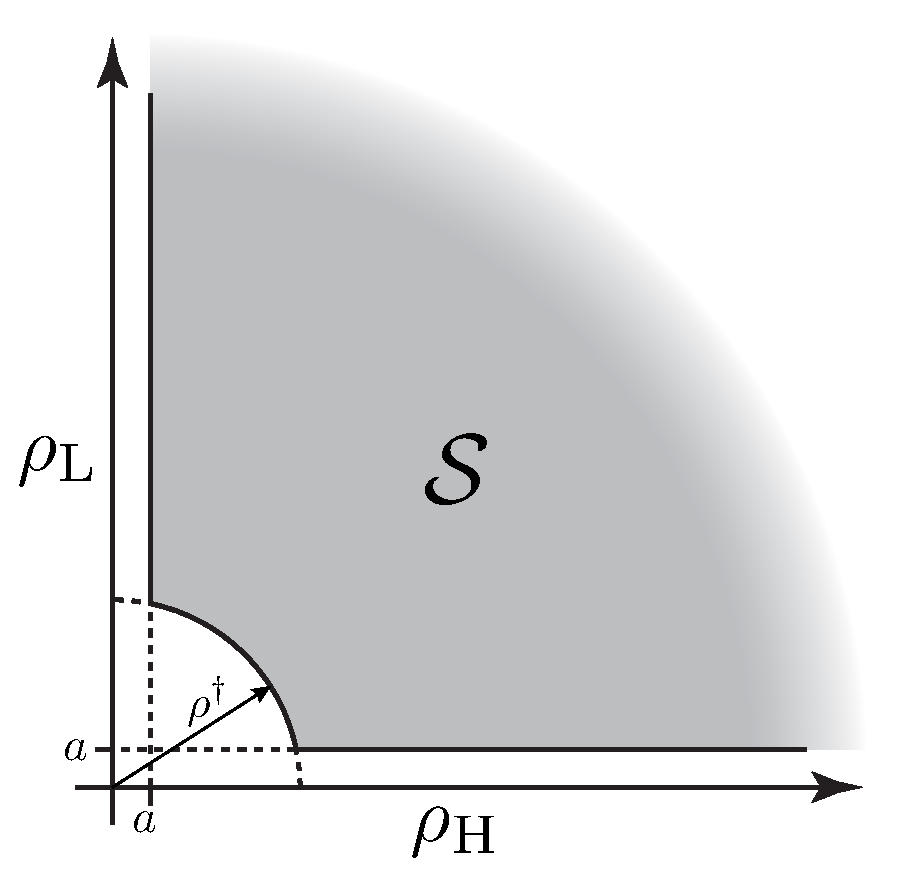
\includegraphics[height=4.25in]{figures/SNRintegrationRegion.pdf} \\
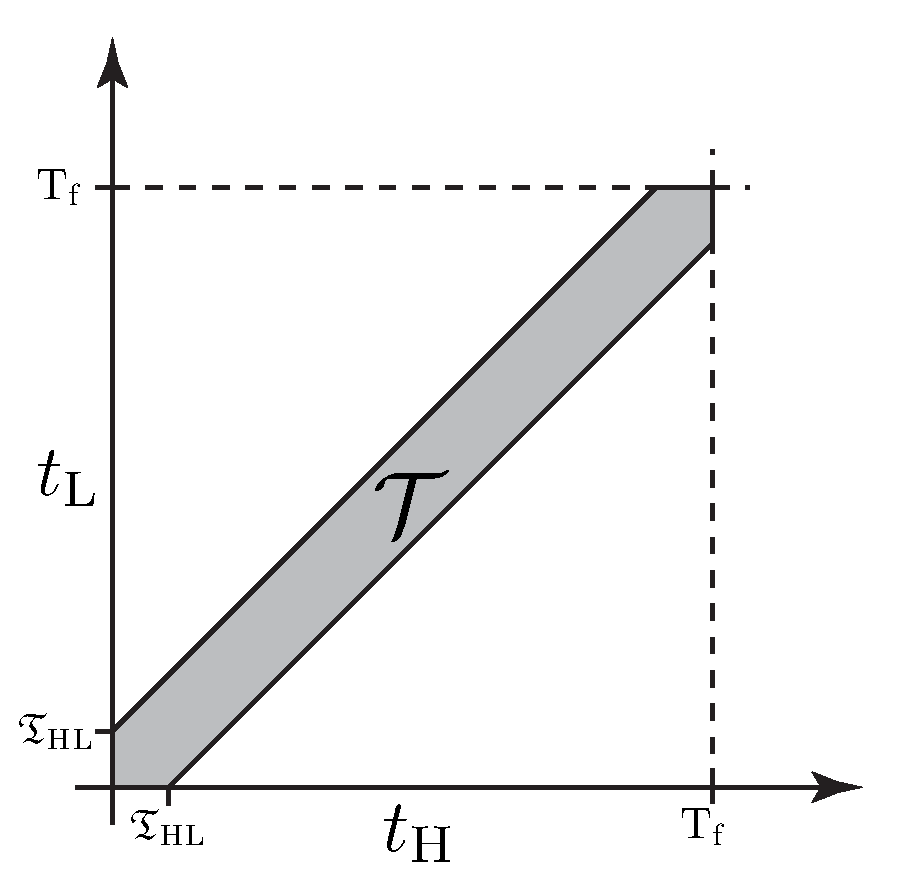
\includegraphics[height=4.25in]{figures/TimeIntegrationRegion.pdf}
\end{center}
\caption{The regions of integration in $\rho$, and time for a network of two detectors, $\varH$ and $\varL$.}
\end{figure}

\if{false}
For example, if we have two arbitrary detectors, $\varH$ and $\varL$, each with two independent sources $\gamma$ and $\delta$, then equation \ref{eqn:N_rate_general} would be:

\begin{eqnarray}
\label{eqn:exampleSources}
\lefteqn{ \mathbb{E}\left(N_{\mathrm{uncorr}}(\rho^{\dagger2} \leq \rho_\varH^2 + \rho_\varL^2, \Tf) \right) } \nonumber \\
 & = &  \vT(\mathrm{T_f}) \int_{\rho_\varH^2 + \rho_\varL^2 \geq \rho^{\dagger2}}  \d \rho_\varH \d \rho_\varL \times \nonumber \\
 & & \left(\rsrc_{\varH,\gamma}P_{\varH,\gamma}(\rho_\varH) + \rsrc_{\varH,\delta}P_{\varH,\delta}(\rho_\varH)\right) \left(\rsrc_{\varL,\gamma}P_{\varL,\gamma}(\rho_\varL) + \rsrc_{\varL,\delta}P_{\varL,\delta}(\rho_\varL)\right) \\ 
 & = & \coincT_{\varH\varL}(2\Tf - \coincT_{\varH\varL})\int_{\rho_\varH^2 + \rho_\varL^2 \geq \rho^{\dagger2}}  \d \rho_\varH \d \rho_\varL \times \nonumber \\
 & & \{ \rsrc_{\varH,\gamma}\rsrc_{\varL,\gamma}P_{\varH,\gamma}(\rho_\varH)P_{\varL,\gamma}(\rho_\varL) + \rsrc_{\varH,\gamma}\rsrc_{\varL,\delta}P_{\varH,\gamma}(\rho_\varH)P_{\varL,\delta}(\rho_\varL) + \nonumber \\
 & & \rsrc_{\varH,\delta}\rsrc_{\varL,\gamma}P_{\varH,\delta}(\rho_\varH)P_{\varL,\gamma}(\rho_\varL) + \rsrc_{\varH,\delta}\rsrc_{\varL,\delta}P_{\varH,\delta}(\rho_\varH)P_{\varL,\delta}(\rho_\varL) \}
\end{eqnarray}

\section{Computing Background Using Time Slides}

Since we wish to find the \ac{FAR}, $\widetilde{\far}$, and not $\widetilde{\RP}_{\mathrm{all}}$, the second (noise/GWs), third (GWs/noise), and fourth (GWs/GWs) terms above are a problem. Admiting gravitational wave sources into the background will give us a higher rate than the true rate $\widetilde{\far}$. The goal, then, is to remove \acp{GW} when computing the background rate.

This presents a problem: we do not know which triggers are due to gravitational waves and which are not (if we did, we would not have to do all this). Worse, the triggers that we are trying to compute false alarm rates for come from the same distribution of single \ac{IFO} triggers as the background rate that we use. To get around these difficulties, we can employ a few things we know about the physics of gravitational waves.

We know that a gravitational wave will arrive at all \ac{IFO}s within the light travel time between them. Therefore if we add some time offset, $\Delta t$ to each detector that is \emph{greater-than} the light-travel time between it and all other detectors but we only allow coincidences from triggers that are \emph{less-than} $\coincT$:
\begin{equation}
\label{eqn:time_constraint}
|t_i - (t_{i+1}+\Delta t)| \le \coincT_{i,i+1},~\Delta t > \coincT_{i,i+1}
\end{equation}
then we cannot get a coincidence from the same gravitational wave in all detectors. Adding the offset only allows gravitational waves that are coincident with \acp{GW} from other sources into the GWs/GWs term in equation \ref{eqn:mixed_source_terms}. While this can still present a problem, if our time searched is much less than the average rate of gravitational waves in the detectors, then the GWs/GWs term effectively goes to zero.

Adding a time offset has the additional advantage that we can repeat the experiment several times using the same data set to get an average value of $\far$, as long as the offet $\Delta t$ is large enough to ensure that each trial, or \emph{slide}, is independent of each other. The duration of each slide is the union of times that the \acp{IFO} are on after the offsets have been applied. If we do $N_{t}$ slides with each slide having duration $t_{k}$, then from equation \ref{eqn:avg_rate_param} we have:

\begin{equation}
\overline{\far} = \frac{\sum_{k=1}^{N_t} N_k\left(\rho^{\dagger2} \leq \sum_{i=1}^{N_d} \rho_i^2, \vec{\mathcal{O}}_k\right)}{\mathrm{T_{b}}}
\end{equation}
where $\mathrm{T_{b}} = \sum_{k=1}^{N_t}t_k$ is the total \emph{background} time. Here we have made the dependence on the time offset in each slide explicit by defining an \emph{offset-vector}:

\begin{equation}
\vec{\mathcal{O}}_k = \left[\Delta t_1 ~ \Delta t_2 ~ \ldots ~ \Delta t_{N_d} \right]_k %  \{\Delta t_i\}_k,~ i = 1, 2, \ldots, N_d
\end{equation}
which gives the time offsets of each detector in the $k^{\mathrm{th}}$ slide. If all the slides have the same duration, $\tau$, then, from equation \ref{eqn:err_R}, the error in the measurement of $\overline{\far}$ is:

\begin{equation}
\delta \overline{\far} = \frac{1}{\tau}\sqrt{\frac{\sum_{k=1}^{N_t} N_k}{N_t}}
\end{equation}

\section{Bias}
\label{sec:bias}

While the time-slide method gives a better estimate of $\far$, it introduces some bias. To quantify this, consider again equation \ref{eqn:N_general} for all sources. For simplicity, we intially consider only a single coincidence window. In this case, the time integral reduces to:

\begin{eqnarray}
\int_{|t_i - t_{i+1}| \le \coincT_{i,i+1}}^{\mathrm{T}=2\coincT_{i,i+1}}\prod_i^{N_d} \d t_i & = & \int_{-\coincT_{i,i+1}}^{\coincT_{i,i+1}} \prod_i^{N_d} \d t_i \nonumber \\
& = & 2 \prod_i^{N_d} \coincT_{i,i+1} \nonumber
\end{eqnarray}
since all points in time will be within the coincidence window. In the $p\th$ slide, equation \ref{eqn:N_general} becomes:

\begin{equation}
\mathbb{E}\left(N_{\mathrm{all}}(\rho^{\dagger2} \leq \sum_i\rho_i^2, 2\coincT )\right) = \int_{\sum_i\rho_i^2 \geq \rho^{\dagger2}} \prod_i^{N_d} \mathbb{E}\left(n_{i,\mathrm{all}}(\rho_i,t_i + \mathcal{O}_p[i] \pm \coincT_{i,i+1} ) \right) \d\rho_i
\end{equation}
To further simplify the problem, we consider the case in which $\rho^\dagger$


If we performed $N_t$ \emph{independent} experiments, then the expected number of triggers in this window would be:

\begin{equation}
\label{eqn:ideal_slides}
N_t \int_{\sum_i\rho_i^2 \geq \rho^{\dagger2}} \d \rho_i \prod_{i}^{N_d} \mathbb{E}( n_{i,\mathrm{all}}(\rho_i, t_i \pm \coincT_{i,i+1}) ) = N_t \int_{\sum_i\rho_i^2 \geq \rho^{\dagger2}} \d \rho_i \prod_{i}^{N_d} \sum_{k=1}^{\infty} k P(k|i,\mathrm{all}; \rho_i, t_i \pm \coincT_{i,i+1})
\end{equation}
When we perform time-slides, however, each of the slides are not truly independent. To see why, focus on one of the detectors, call it $\varH$, against which the other detectors are slid. In the first slide, the integrand is equation \ref{eqn:ideal_slides} (with $N_t = 1$). In each subsequent slide, the same expression will hold for all detectors aside from $\varH$, since, by sliding, we have introduced new data into the coincidence window. Yet because we are using the \emph{same} data in $\varH$, the probability of getting $k$ triggers in $\varH$ is \emph{not} $P(k|\varH,\mathrm{all}; \rho_i, \tau)$; instead, it is one if $k = n^{(0)}_{\varH}$ --- where $n^{(0)}_{\varH}$ is the number of triggers that occurred in $\varH$ in the first slide --- and zero otherwise. In other words, the \ac{PDF} in $\varH$ has collapsed around $n^{(0)}_\varH$. The expected number in the coincidence window is thus:

\begin{equation}
\label{eqn:actual_slides}
N_t \left(\prod_{i \neq \varH} \sum_{k=1}^{\infty} k P(k|i,\mathrm{all}; \rho_i, t_i \pm \coincT_{i,i+1})\right) \sum_{k=1}^{\infty} k \delta^{k}_{n^{(0)}_\varH} = N_t \prod_{i \neq \varH}^{N_d} \mathbb{E}( n_{i,\mathrm{all}}(\rho_i, t_i \pm \coincT_{i,i+1}) ) n^{(0)}_\varH
\end{equation}



%%%%%%%%%%%%%%%%%%%%%%%%%%%%
\if {false}
$m^{\mathrm{th}}$ noise source in the \varH~ detector and the $n^{\mathrm{th}}$ noise source in \varL. Let the true rate densities of these noise sources be $\widetilde{r}_{\varH,m}$ and $\widetilde{r}_{\varL,n}$, respectively. At a given time $t$, we will get a coincident trigger if there is at least one trigger from each source within $\coincT_{\varH\varL}$. The probability of getting atleast one coincident trigger is therefore:

\begin{eqnarray}
P(N_c \geq 1 | \widetilde{\rsrc}_{\varH,m}, \widetilde{\rsrc}_{\varL,n}, t \pm \coincT_{\varH\varL} ) &  & \nonumber \\
 & = & P(N \geq 1 | \widetilde{\rsrc}_{\varL,m},t \pm \coincT_{\varH\varL})P(N \geq 1 | \widetilde{\rsrc}_{\varL,m}, t \pm \coincT_{\varH\varL}) \nonumber \\
 & = & \left( 1 - e^{-\widetilde{\rsrc}_{\varH,m}2\coincT_{\varH\varL}} \right)\left( 1 - e^{-\widetilde{\rsrc}_{\varL,m}2\coincT_{\varH\varL}} \right)
\label{eqn:true_coinc_prob}
\end{eqnarray}
In equation \ref{eqn:true_coinc_prob} we have used the fact that the probability of getting one or more events from a Poisson distribution is:

\begin{eqnarray}
P(N \geq 1 | \RP, \tau) & = & 1 - P(0|\RP,\tau) \nonumber \\
    & = & 1 - e^{-\RP\tau}
\end{eqnarray}

Within a single slide, each block of coincident time can be considered to be an independent measure of the coincident $m,n$ rate density $\far_{m,n}$. Assuming $\far_{m,n}$ is constant across the duration of the slide, $\tau$, then we have $\tau/\coincT_{\varH\varL}$ measures of $\far_{m,n}$. However, this will not be sufficient to get a good approximation of $\widetilde{\far}_{m,n}$ especially if:

\begin{equation}
\widetilde{r}_{\varH,m}\widetilde{r}_{\varL,n} \left(\frac{\tau}{\coincT_{\varH\varL}}\right) < \frac{1}{\coincT_{\varH\varL}^2}
\end{equation}
In this case the expected number of events across the slide would be less than 1, making it likely that we would record no value and therfore end up with a mean value of zero for $\overline{\far}_{mn}$. For this reason, we extend the number of measures of $\far_{mn}$ we have by adding more slides.

However, the slides are not true indepedent measurements. Consider the same point in time in the $\varH$ detector as before, but now in the next slide. If this was a truly independent measurement, then the probability of getting one or more coincident triggers would again be equation \ref{eqn:true_coinc_prob}. The probability of getting a trigger during this period of time in $\varL$ would be the same it has been slid a period of time greater than $\coincT_{\varH\varL}$. The probability of getting a trigger in $\varH$, however, is \emph{not} the same. Since we are using the exact same period of time, it will be either 0 or 1, depending on whether or not we got a trigger in the first slide. Thus, the probability of getting a trigger at time $t$ for this and all subsequent slides is:

\begin{eqnarray}
P(N \geq 1|\widetilde{\rsrc}_{\varH,m}, \widetilde{\rsrc}_{\varL,n}, t \pm \coincT_{\varH\varL}, \mathcal{O}_{k \neq 1}) &  \nonumber \\
 = & \left\{
\begin{array}{l l}
1 - e^{-\widetilde{\rsrc}_{L,n}\coincT_{\varH\varL}} & \mbox{if $N_{\varH,m}(\mathcal{O}_1) \geq 1$} \\
0 & \mbox{if $N_{\varH,m}(\mathcal{O}_1) = 0$}
\end{array}
\right.
\end{eqnarray}

\fi
%In our ideal world of independent measurements, the probability that we will get atleast one coincident trigger with $\rho_c^2 \geq \rho^{\dagger2}$ at a time $t$ is given by the probability that we get one or more trigger in each detector within $\coincT$:

%\begin{equation}
%P(N \geq 1 | t, \{\widetilde{r}_{i,j}\}) = \prod_{i = 1}^{N_d} P(N \geq 1 | t\pm\Delta \coincT_{i}, \widetilde{r}_{i,n_i})
%\end{equation}

\fi

\end{document}

\fi

\end{document}
